\documentclass[a4paper,11pt,fleqn]{jbook}
%\documentclass[a4paper,11pt]{jarticle}
%\usepackage{u-thesis}
\usepackage{u-thesis-p}
\usepackage{graphicx}
\usepackage{amsmath}
\usepackage{mediabb}%pdf

\usepackage{ascmac}
\usepackage{here}
\usepackage{txfonts}
\usepackage{listings,jlisting}


% title
\title{LLVMコンパイラ基盤を用いた}
\titletwo{ベクトル化コード生成についての検討}
\author{永池 晃太朗}
\kind{卒業論文}  % 卒業論文
\date{2022年3月}
\lab{宇都宮大学工学部}
\labtwo{情報工学科}
\id{XX-XX}  % 学科から指定された番号をいれる

\etitle{Consideration of Vectorized Code Generation}
\etitletwo{Using LLVM Compiler Infrastructure}
\eauthor{Kotaro Nagaike}

\begin{document}

\maketitle

\begin{jabstract}
従来のSIMD命令では同時演算数を変更する場合,それに応じて機械語コードを作り直す手間があった.
そこで,データ並列処理のために機械語コードの変更なく,同時演算数を変更できるスケーラブルなベクトル拡張を実現したベクトル拡張付きRISC-Vが開発された.ベクトル拡張付きRISC-Vではプレディケートレジスタを用いたベクトル処理を行うことによってスケーラブルなベクトル拡張を実現している.
しかし,このベクトル拡張に対応したコンパイラがないため,ベクトル拡張付きRISC-Vのアセンブリコードを生成できないという問題点がある.これに対する解決策としてベクトル拡張付きRISC-Vに対応したコンパイラの開発を検討した.コンパイラ基盤であるLLVMを用いて既に実装済みのRISC-V向けコンパイラの機能を再利用すればコンパイラを一から開発するより容易にアセンブリコードの生成を行うことができる.また,LLVMの機能である自動ベクトル化を用いることでベクトル化されたコードの生成が可能であることから,LLVMを用いることによってベクトル拡張付きRISC-V向けにアセンブリコードを得ることができると考えた.

本論文ではLLVMコンパイラ基盤におけるコード生成について述べ,そのコード生成において用いられる命令の定義手法から,独自命令生成のための命令定義を行った.独自命令の定義として命令フォーマット,出力する命令ニーモニックについて定義を行う.そして,ベクトル化されたLLVM中間表現であるLLVM IRから独自命令の生成を可能としている.

本論文ではベクトル拡張付きRISC-Vの命令の内,ベクトル算術・論理演算命令,即値を用いるシフト命令の実装について述べる.

更に,実装した命令が正常に入力ソースコードから生成されることを確認する.C言語を用いて配列加算等のプログラムを作成し,そのプログラムのアセンブリコードの生成を行う.

また,現段階では実装できていない命令として,ベクトルロード・ストア命令等がある.その命令生成に向けて新たに必要な定義や変更点などについて述べる.
\end{jabstract}

%abstract
\begin{abstract}
For processing that performs the same operation on multiple data, such as image processing, it is possible to achieve higher speed by using data parallel processing with SIMD instructions that process multiple data with a single instruction.
However, when using SIMD for data parallel processing, the number of simultaneous operations, which is the number of data to be processed in one instruction, is fixed for SIMD instructions. Therefore, if the number of concurrent operations is changed to improve the processing performance, the machine language code must be rewritten.
To solve this problem, RISC-V with vector extension has been developed for data-parallel processing, which is a scalable vector extension that can change the number of concurrent operations without changing the machine code. RISC-V with vector extension is an extension of RISC-V processor with vector processing capability. The RISC-V with vector extension uses predicate registers for vector processing to achieve scalable vector extension.
However, there is a problem that the assembly code of RISC-V with vector extension cannot be generated because there is no compiler that supports this vector extension. As a solution to this problem, we study how to realize a compiler that supports RISC-V with vector extensions. By using LLVM, which is a compiler infrastructure, and reusing the functions of already implemented compilers for RISC-V, it is easier to generate assembly code than developing a compiler from scratch. In addition, the automatic vectorization function of LLVM can be used to generate vectorized code, so we believe that assembly code for RISC-V with vector extensions can be obtained by using LLVM.

In this paper, we describe the code generation in the LLVM compiler infrastructure and define instructions for generating original instructions. Among the instructions of RISC-V with vector extensions, we describe the implementation of vector arithmetic and logic instructions and shift instructions using immediate values.
In addition, we confirm that the implemented instructions can be successfully generated from the input source code, and show that programs such as array addition written in C can be used to generate their vectorized assembly code.
We will also show that the vectorized assembly code can be generated using programs such as array addition written in C. There are instructions such as vector load/store instructions that have not been implemented at this stage. In this paper, we describe the definitions and changes required to generate such instructions.    % 同一ディレクトリのabstract.texが読み込まれる
\end{abstract}

\newpage
\tableofcontents    % 目次


\newpage
\chapter{はじめに}
\label{chp:intro}   % ラベルを貼っておくと後々便利
%intro.tex
FPGA (Field Programmable Gate Array)はユーザによって回路の再構成が可能なLSIであり,目的の処理をハードウェアとして実装可能なデバイスである.
近年FPGAの大容量化,高性能化によって大規模な回路が実現可能になった.これによりFPGAは自動運転を始めとする組込み分野での利用増加が期待されている.

FPGAを用いたハードウェア開発はHDL (Hardware Description Language)によるRTL(Register Transfer Level)設計が広く用いられている.RTLはFPGA上に構成する回路の信号の流れや制御構造を直接設計できる一方,動作検証やデバックが難しく,短期間で複雑な処理の開発は困難である\cite{bib:fpga}.
そのため,FPGAによる開発期間を短縮する方法として,専用ハードウェアとプロセッサを用いたソフトウェアによる処理を組み合わせる方法が考えられる.FPGA上のハードウェアリソースを用いて実装するプロセッサのことをソフトコアプロセッサという.
一般的に組込みシステムではそのコストやサイズ,消費電力などに制限があるためハードウェア資源に制約があることが多く,メモリバンド幅が限られることからメモリシステムの性能が高くないことが多い.メモリシステムの性能が低いと演算性能を高くしてもメモリアクセスに時間がかかり,結果としてシステム全体の性能はメモリシステムの性能によって左右される\cite{bib:2}.
そこで,ソフトコアプロセッサによる処理を考える.すべての処理を専用ハードウェア回路で行うのではなく,高い性能の求められない汎用的な処理についてはソフトコアプロセッサにて行うことにより開発する専用ハードウェア回路を削減でき,ソフトコアプロセッサの性能が向上して専用ハードウェア回路を削減しても求められた性能に達することができればハードウェアの開発コストを抑えることができる.

組込み分野ではAI技術に注目が集まっている.独立行政法人情報処理推進機構の調査によると,将来強化/新たに獲得したい技術として組込み/IoT関連企業の46\%がAI技術を挙げている\cite{bib:ipa}.

AI技術の応用としては画像認識などの画像処理が行われる.画像処理では画像を構成する画素に対して同じ処理を行うようなものが多い.このように複数のデータに対して同じ演算を行う処理については,単一命令で複数データの処理を行うSIMD (Single Instruction, Multiple Data)や,複数命令を並列に実行するMIMD (Multiple Instruction, Multiple Data)による並列処理で高速化が可能である\cite{bib:simd_mimd}.
MIMDは複数の制御を並列化することができるため,異なる処理を同時に実行するアプリケーションでは有効である.しかし,プロセッサに複数の制御ユニットをもたせる必要があるためSIMDと比較するとハードウェアのコストが大きくなる.一方SIMDは単一の制御ユニットで複数の演算ユニットを並列動作させるため制御ユニットのコストは低くなる.
データ並列処理では複数のデータに対して同じ処理を実行するためSIMDによって並列処理が可能である.

SIMDによる並列処理を行う場合,SIMD命令は1命令で演算するデータ数が決まっている.そのため演算性能を上げるために同時演算数を変更すると機械語コードを作り直す必要がある.異なる同時演算数でも同一の機械語コードを利用可能とするためには,機械語コードが同時演算数に依存しないスケーラブルなベクトル拡張が必要である.スケーラブルなベクトル拡張により機械語コードを変更することなく,必要に応じて容易に同時演算数を増やし高性能化することが可能となる.

スケーラブルなベクトル拡張を実現したものとしてオープンな命令セットアーキテクチャであるRISC-V\cite{bib:risc-v}をベクトル拡張したベクトル拡張付きRISC-V\cite{bib:kimura}が提案されている.ベクトル拡張付きRISC-Vは組込み機器に広く用いられているARMのベクトル拡張であるARM SVE (Scalable Vector Extension)\cite{bib:arm_sve}の命令セットを参考に組み込み向けにRISC-Vに拡張したものである.しかし,ベクトル拡張付きRISC-Vに対応したコンパイラが存在していない.そこで解決策としてベクトル拡張付きRISC-Vのベクトル命令のアセンブリコードを得るためのコンパイラの開発を検討した.

本論文では,第2章で現在のMIQSプロセッサについて述べる.第3章でベクトル拡張付きRISC-V命令の生成のために利用したコンパイラ基盤であるLLVM\cite{bib:llvm}について述べる.第4章で実際に命令生成のための実装について述べる.第5章では実際のソースコードからアセンブリコードの出力を行った結果について述べる.


\newpage
\chapter{MIQSプロセッサ}
\label{chp:2}
%2.tex

本章ではSIMD演算機能を持つソフトコアプロセッサであるMIQSプロセッサについて述べる.


\section{RISC-V}
\label{chp:2_1}
%2.1.tex

RISC-Vはカルフォルニア大学バークレイ校が新たに開発したRISCの設計思想に基づく命令セットアーキテクチャ(ISA)である.RISC-VはオープンなISAであり,ライセンスが不要である.

従来のISAでは,後方バイナリ互換性を維持するために過去に拡張した命令すべてを実装する必要がある.しかし,このようなISAでは命令数が増加し複雑になる.そこでRISC-Vではモジュール式ISAを採用している.\cite{bib:risc-v-module}
RISC-Vのシステムの機能を独立したモジュールとして分け,アプリケーションに応じて拡張機能を組み込むかを選択できる.RISC-Vには必ず組み込まなければならない基本命令セット(RV32I)の他に,主な拡張機能として乗算及び除算(RV32M),単精度浮動小数点(RV32F),倍精度浮動小数点(RV32D)等がある.

RISC-Vの基本命令は6つの命令フォーマットで表すことができる.基本命令の命令フォーマットを図\ref{fig:RISC-V_Instruction_formats}
に示す.

\begin{figure}
    \centering
    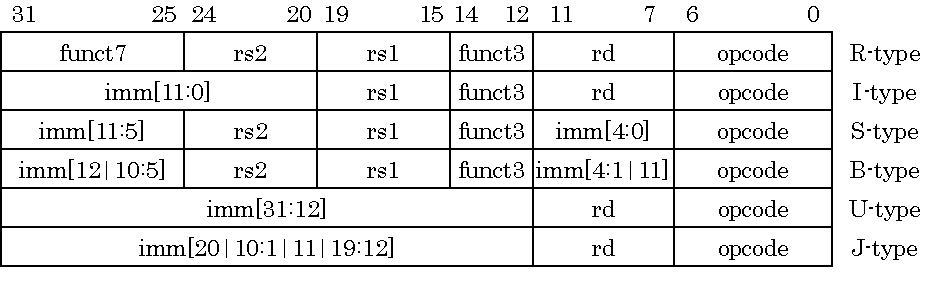
\includegraphics[scale=0.8]{image/Inst_Format.pdf}
    \caption{基本命令の命令フォーマット}
    \label{fig:RISC-V_Instruction_formats}
\end{figure}

R形式は2つのソースレジスタを扱う形式,I形式は12ビットの即値を扱う命令,S形式はストア命令,B形式は条件分岐命令,U形式は20ビットの即値を扱う命令,J形式は無条件ジャンプ命令の形式である.命令形式が単純であるため命令のデコーディングが単純化される.
\section{MIQS概要}
\label{chp:2_2}
%2.2.tex
ベクトル拡張付きRISC-Vプロセッサとは,RISC-Vコアにベクトル演算機能を拡張したソフトコアプロセッサである.
図\ref{fig:MIQS_system}
にベクトル拡張付きRISC-Vプロセッサの全体構成を示す.ベクトル拡張付きRISC-VプロセッサのRISC-VコアプロセッサはRISC-Vプロセッサを使用している.このプロセッサはVerilog-HDLで記述された5段パイプラインプロセッサで必要最低限の基本命令セットであるRV32Iで規定された命令を実装している.

\begin{figure}[b]
\begin{center}
    
\includegraphics[scale=1.2]{image/MIQS_system.pdf}
    \caption{ベクトル拡張付きRISC-Vプロセッサの構成}
    \label{fig:MIQS_system}
\end{center}
\end{figure}

命令のフェッチおよびデコードはRISC-Vコアプロセッサ上で行い,デコード結果がベクトル拡張命令であったときはベクトル処理ユニットで動作させる.

メモリアクセスに関しては,プロセッサからメモリコントローラを介してSDRAMにアクセスする.メモリアクセス要求がプロセッサから発行されたときは,メモリコントローラがSDRAMを制御してメモリアクセスを実現する.また,ベクトルメモリアクセスに関してもメモリコントローラにて行う.
SDRAMコントローラとメモリコントローラ間のデータバス幅は128ビットであるから,プロセッサとメモリコントローラ間のデータバス幅は128ビットとなっている.

RISC-Vコアプロセッサは命令フェッチ (IF),命令デコード (ID),実行 (EX),メモリアクセス (MA),ライトバック (WB)の5段のパイプラインで構成されている.
%ベクトル処理ユニットはベクトル長を256ビット,データの型は32ビット整数型を想定して設計されている.
ベクトル処理ユニットとRISC-Vコアの双方で動作する必要のある命令に対応するためベクトル処理ユニットはRISC-Vコアと同じく5段パイプライン構成となっており,RISC-Vコアと協調動作する構成となっている.なお,命令フェッチ部分と命令デコード部分はRISC-Vコアと共通となっている.

ベクトル拡張付きRISC-Vプロセッサによってスケーラブルなベクトル拡張を実現し,同時演算数の変更による機械語コードの変更の必要がなくなったが,ベクトル拡張付きRISC-Vプロセッサが対応している命令セットのアセンブリコード等を出力できるコンパイラがない.アセンブリコードを生成する手段として,インラインアセンブラを利用する方法が考えられる.インラインアセンブラを利用する場合,アセンブラプログラミングの知識を必要とする他,コンパイラの最適化の影響で問題が起きる場合がある.その場合,volatile修飾子の利用によりコンパイラの最適化からインラインアセンブラ記述部分を対象外とすることで問題を回避できるが,volatile修飾子の利用は他の部分の最適化に悪影響を及ぼすことがある.また,カスタム命令の追加をした場合,命令のスケジューリングや追加レジスタに対するレジスタ割り当てを行うことができない.
intrinsics関数を用いる手法も考えられるが,intrinsics関数によって記述されたソースコードはベクトル拡張付きRISC-V以外では利用できない.そのためベクトル拡張付きRISC-Vのためにソースコードを記述する必要がある.
そのため,既存のコンパイラの機能を再利用してベクトル拡張付きRISC-V命令のアセンブリコードを生成可能なコンパイラを開発する手法を検討する.
\section{ベクトル拡張付きRISC-V}
\label{chp:2_3}
%2.3.tex
ここは\ref{chp:2_3}節です.



\newpage
\chapter{LLVM}
\label{chp:3}
%3.tex
\ref{chp:3}章! 黙々と書こう.

\section{LLVM概要}
\label{chp:3_1}
%3.1.tex
LLVMは2000年にイリノイ大学で開発が開始されたコンパイラ基盤である.コンパイラ基盤とはコンパイラに必要となるモジュールをまとめたもので,コンパイラを開発するためのフレームワークである.
LLVMの構成を図\ref{fig:LLVM}に示す.LLVMはソースコードをLLVMの中間表現であるLLVM IRに変換するフロントエンド,LLVM IRに対して最適化等の操作やLLVM IRから機械語やアセンブリコードへの変換を行うバックエンドに分かれている.中間表現であるLLVM IRは階層構造のドメイン固有言語である.
LLVMではこれらの機能がモジュール化されており,独自機能を実装する以外は既存のものを再利用することができる.例えば新たなアーキテクチャ向けのコンパイラを開発する際はバックエンドのみ実装を行い,フロントエンドについては再利用することができる.

\begin{figure}[tb]
    \centering
    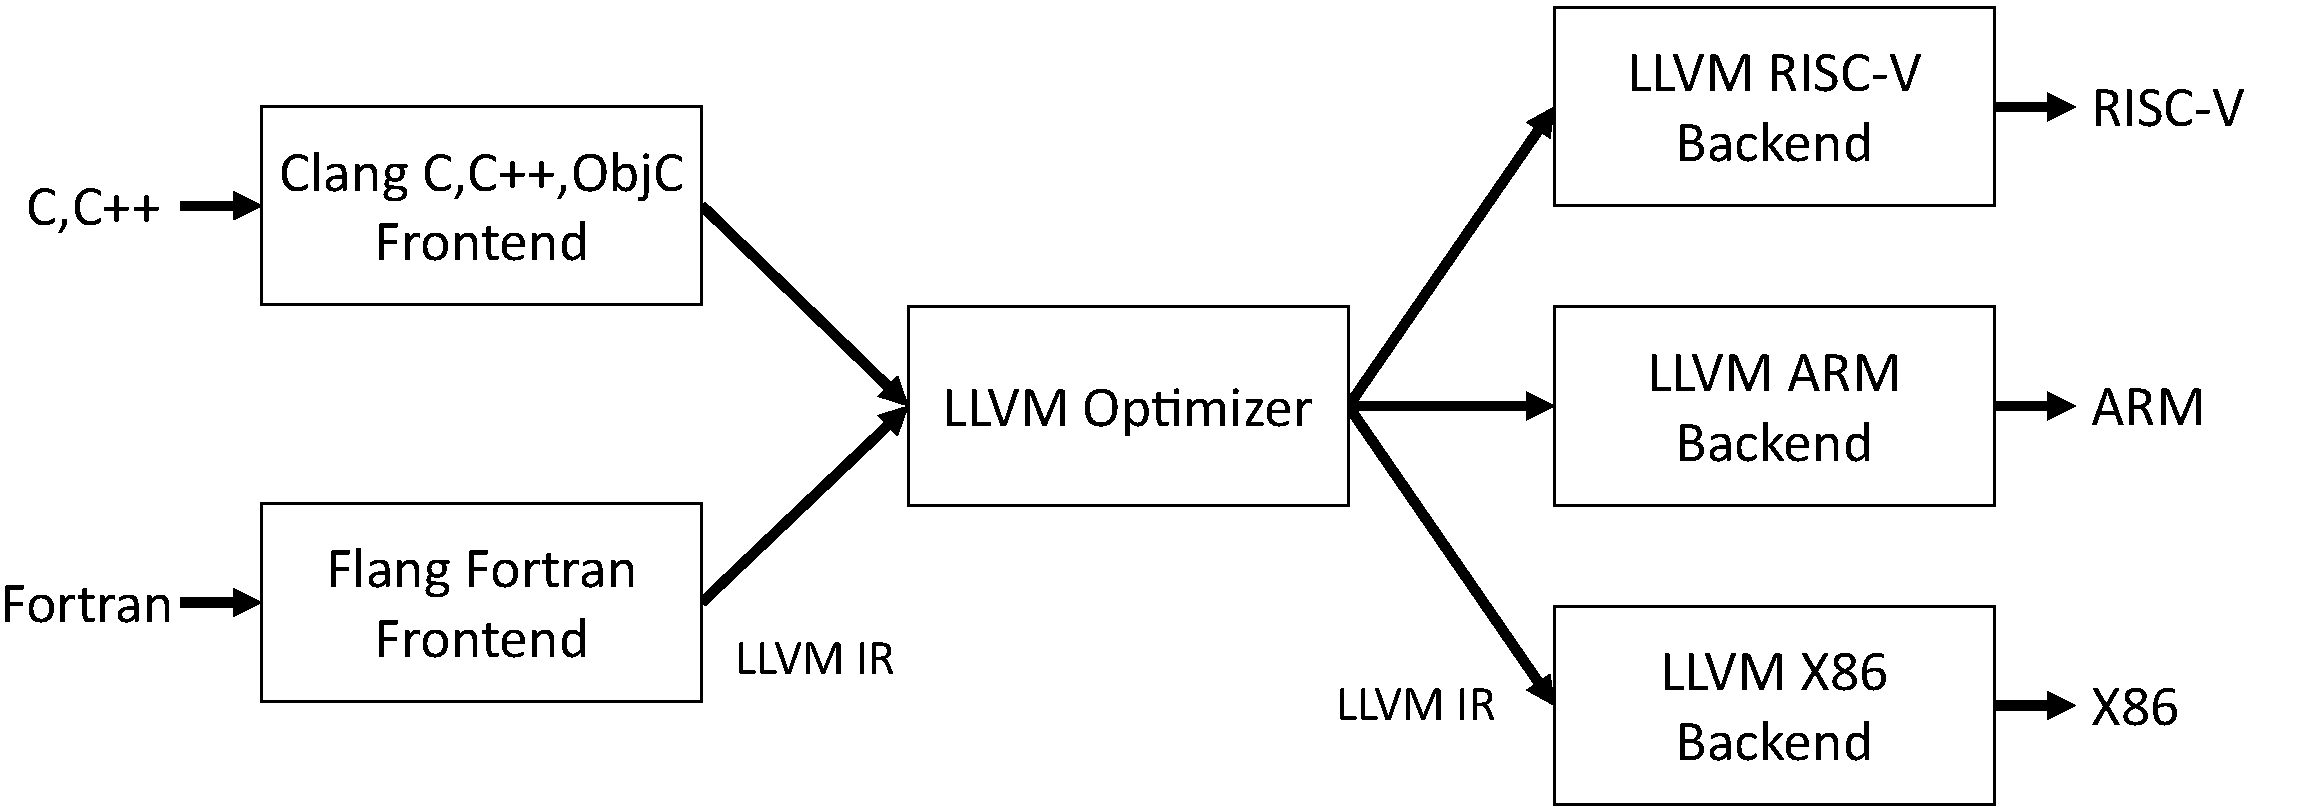
\includegraphics[scale=0.4]{image/LLVM.pdf}
    \caption{LLVMの構成}
    \label{fig:LLVM}
\end{figure}

LLVMには既にRISC-Vを対象としたコード生成のためのバックエンドが実装されている.本研究ではRISC-Vを独自にベクトル拡張したベクトル拡張付きRISC-Vの命令の生成を目的としているため,このRISC-V向けのバックエンドに対して変更を加えることによって独自命令の生成を行う.

LLVMバックエンドにおけるコード生成の流れを図\ref{fig:LLVM_backend}に示す.
LLVMバックエンドではPassによって処理が行われる.図\ref{fig:LLVM_backend}
ではLLVMバックエンドにおけるデータフォーマットの変化と実行されるPassを表している.

\begin{figure}[tb]
    \centering
    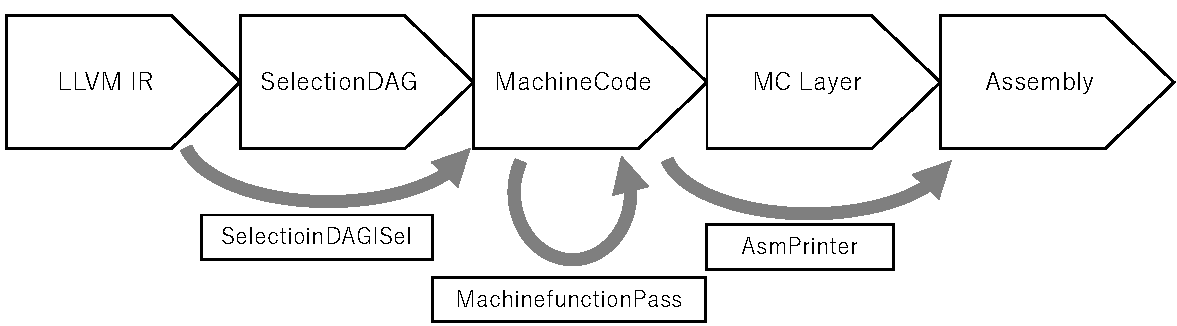
\includegraphics[scale=0.7]{image/backend.pdf}
    \caption{LLVMバックエンド}
    \label{fig:LLVM_backend}
\end{figure}

バックエンドではLLVM IRからDAG(Directed Acyclic Graph)であるSelectionDAGへフォーマットを変換する.SelectionDAGはLLVM IRをグラフ形式で表したもので,各命令やデータの依存関係を表現する.SelectionDAGへの変換はSelectionDAGISelパスで行われ,SelectionDAGは最終的にSelectionDAGISelパスによってMachineCod形式に変換される.SelectionDAGISelではLower,Combine,Legalize,Select,Scheduleのフェーズから構成される.

LowerはLLVM IRからSelectionDAGに変化させるフェーズである.このフェーズではLLVM IRからSelectionDAGのノードへと一対一の対応を行う.この段階ではターゲットマシンでは利用できない命令やデータ形式を含んでる不正(illegal)な状態である.

Combineフェーズではパターンマッチングによる置き換えで最適化を行い,命令の単純化を行う.

Legalizeはターゲットマシンではサポートされていない命令やデータ形式を他のものに置き換えるフェーズである.このフェーズによって不正な状態であったSelectionDAGノードが正当(legal)な状態となる.

SelectフェーズではSelectionDAGのノードをターゲットマシンの命令を含んだMachineNodeへと変換する.

Scheduleフェーズでは構築されたグラフの依存関係を元に命令をスケジューリングするフェーズである.

SelectionDAGISelパスではこれらのすべてのフェーズが終わった後にMachineCodeを出力する.

MachinefunctionパスではMachineCodeという形式を扱う.この形式はLLVM IRと似た構成になっているが,より機械語に近い表現になっている.
MachineCodeがSelectionDAGISelによって生成された直後はまだ命令で扱うレジスタは無限個あると仮定した仮想レジスタやphi関数を含んだSSA(Static Single Assignment form)形式で表現されている.MachinefunctionPassではレジスタの割当やphi命令の削除を行い,MachineCodeを非SSA形式へと変換する.

AsmPrinterパスはMachineCodeをMC Layer形式へと変換した後にアセンブリコードなどを出力するパスである.MC Layer形式はMachineCode形式のような階層構造がない形式であり,アセンブリコードへの変換だけでなく,オブジェクトファイルへの変換のための形式である.


\section{LLVMによる自動ベクトル化機能}
\label{chp:3_2}
%3.2.tex

LLVMには自動ベクトル化機能が備わっている.
自動ベクトル化とは配列の演算処理などのループによる繰り返し処理をベクトル命令の形式に置き換える機能である.LLVMによる自動ベクトル化機能はソースコードにおけるループをベクトル化されたLLVM IRへと変換が行われる.
LLVMによる自動ベクトル化の例を図\ref{fig:LLVM_auto_vec}に示す.
LLVM IRにおいてベクトル命令はベクトル型を用いて表現される.図\ref{fig:LLVM_auto_vec}にて<128 x i32>となっている箇所がベクトル型の指定を行っており,これは128個の32ビット整数の演算を行うベクトル型の命令となっている.

\begin{figure}[b]
    \centering
    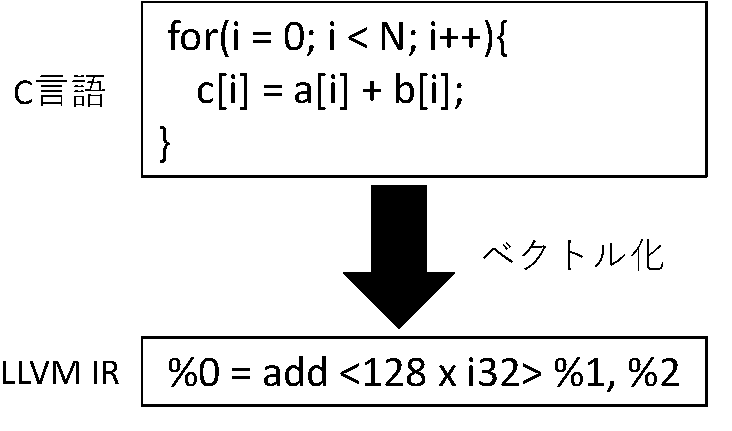
\includegraphics[scale=0.7]{image/Auto_vectorize.pdf}
    \caption{LLVMによる自動ベクトル化例}
    \label{fig:LLVM_auto_vec}
\end{figure}

%また,LLVM IRにおけるベクトル処理の流れを図%フローチャートを作って載せる
%に示す.
また,LLVM IRでは対象の全データに演算を行うための制御を行っている.例えば対象データ要素数が400とし,一度にベクトル演算を行う個数を128とする.この場合,128個を対象としたベクトル演算を3回行う.するとベクトル演算では384個の要素を演算することができるが,16個の要素が余っている.このあまりに関しては逐次処理によってスカラ演算を16回繰り返す処理を行う.これによってすべてのデータの演算を可能にしている.

LLVMではベクトル化されたLLVM IRからベクトル命令を生成することが可能であるが,RISC-VのV拡張命令の生成については現在実験段階であり,完全なアセンブリコードを得ることはできない.

\newpage
\chapter{ベクトル拡張付きRISC-Vコンパイラ}
\label{chp:4}
%4.tex

本章ではベクトル拡張付きRISC-Vのベクトル命令をLLVMによって生成するための命令実装手法と,実際に実装した命令の定義について述べる.
\section{LLVMバックエンドにおける独自命令実装手法}
\label{chp:4_1}
%4.1.tex

LLVMにおいて特定のターゲットマシン命令の生成は\ref{chp:3_1}で述べたSelectionDAGISelパスによるSelectフェーズにてLLVM IRの命令からターゲットマシン命令に変換されることによって行われる.
この変換はSelectionDAGのノードに対してパターンマッチングを行い,特定のパターンにターゲット命令を対応させる手法で行われる.

このパターンマッチングに用いるパターンはLLVMの固有ドメイン言語であるTableGenによって行われる.TableGenはターゲットマシンの命令やレジスタ等の情報を記述するために用いられる.TableGenでは命令生成のためにパターンの定義だけでなく,アセンブリコード等の出力のためにニーモニックの定義や命令フォーマットの定義も行っている.

SelectionDAGのパターンマッチングの例を図\ref{fig:SelectionDAG_example}
に示す.
図\ref{fig:SelectionDAG_example}
では加算命令の例を示している.図\ref{fig:SelectionDAG_example}上にパターン定義クラスPatがある.Patクラスの第一引数と変換前のSelectionDAGのノードが一致した場合,Patクラスの第二引数で指定したノードに変換する.

\begin{figure}[bt]
    \centering
    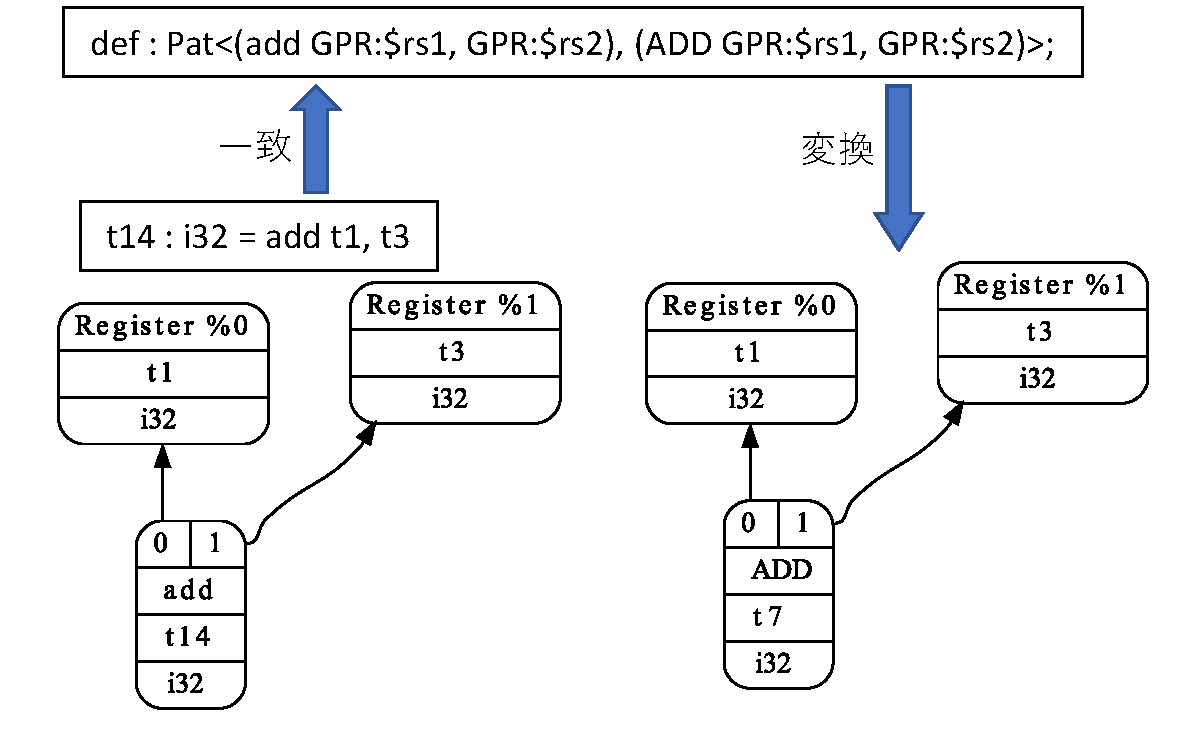
\includegraphics[scale=0.6]{image/SelectionDAG_example.pdf}
    \caption{SelectionDAGの命令変換}
    \label{fig:SelectionDAG_example}
\end{figure}

この様にSelectionDAGのパターンと命令ごとに定義されているパターンが一致したときに対応した命令にノードが変換される.
LLVMではRISC-VのV拡張命令のためのパターン定義が既に実装されており,そのパターンと一致した際に変換する命令を独自のベクトル拡張付きRISC-Vの命令に定義しなおすことによってベクトル拡張付きRISC-V命令の生成を実現する.

LLVMにおける命令の定義は命令フォーマットの定義と命令の定義に分かれる.命令フォーマットはTableGenによって命令の種類ごとにフォーマットのクラスを定義を行う.LLVMにおける命令フォーマットは基本クラスRVInstを継承する形で行われる.RVInstでは32ビットのフィールドInstや命令のニーモニックを格納するAsmStringを定義している.このRVInstを継承して異なるフォーマットを定義していく.

命令の定義は命令フォーマットのクラスをインスタンス化する形で行われるが,そのために命令フォーマットを更に継承したクラスを定義する.このクラスは似たような種類の命令を定義するに当たって同じような定義を何度も繰り返さないように定義する.

命令フォーマット,命令定義のクラスの継承関係を図\ref{fig:InstFromat_class}%図を作り直し、ラップクラスも書く
に示す.基本クラスであるRVInstを継承して基本命令のフォーマットの定義を行っている.クラスALU\_rr,ALU\_riはそれぞれ算術演算命令のためのクラスである.ALU\_rrは汎用レジスタ同士の加算や減算の算術演算の定義に用いられ,ALU\_riは即値を用いた算術演算の命令定義に用いられる.

\begin{figure}[tb]
    \centering
    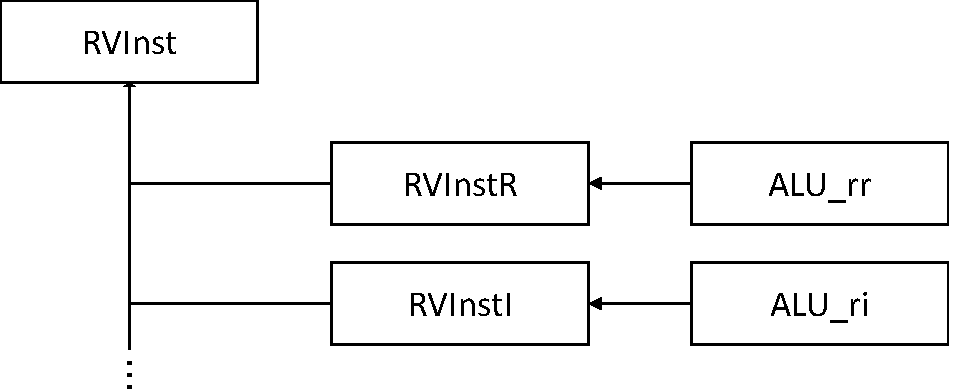
\includegraphics[scale=0.5]{image/InstFormat_class.pdf}
    \caption{基本命令フォーマットクラス継承関係}
    \label{fig:InstFromat_class}
\end{figure}
\section{ベクトル拡張付きRISC-V命令の定義}
\label{chp:4_2}
%4.2.tex

\ref{chp:4_1}で述べたLLVMのRISC-Vバックエンドでの命令生成のための命令定義クラスについて,ベクトル拡張付きRISC-Vのベクトル命令のための命令フィールドと命令の定義を行った.

図\ref{fig:MIQSInst_class}
に定義した命令フィールド定義クラスと命令定義のためのクラスの継承関係を示す.

\begin{figure}[tb]
    \centering
    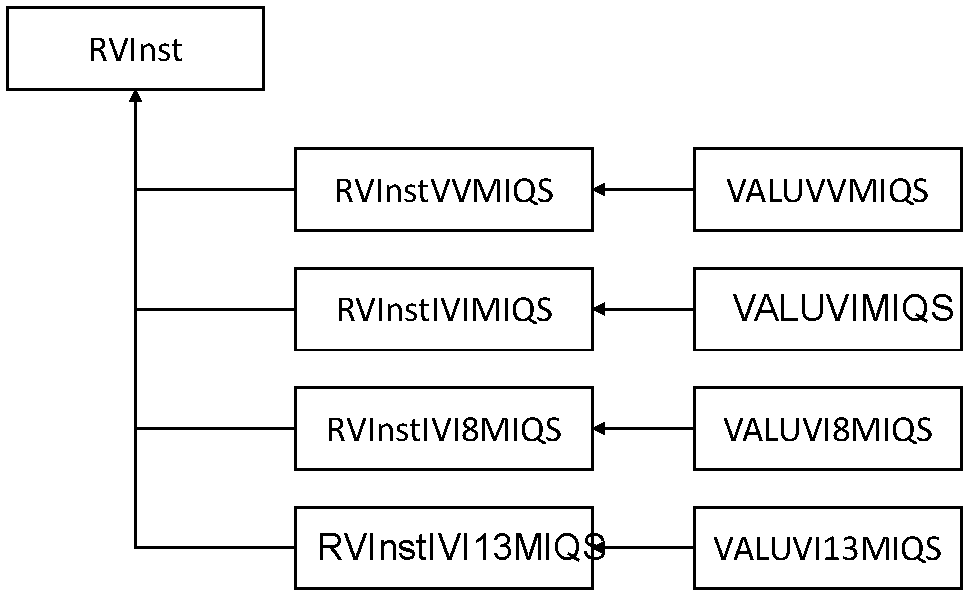
\includegraphics[scale=0.6]{image/MIQSInst_class.pdf}
    \caption{定義したクラスの継承関係}
    \label{fig:MIQSInst_class}
\end{figure}

本研究ではベクトル拡張付きRISC-Vの命令のうち,ベクトル演算命令のプレディケートレジスタを用いない命令を実装した.

実装した命令とそのフォーマットを図\ref{fig:jissou_inst_format}
にまとめる.

\begin{figure}[tb]
    \centering
    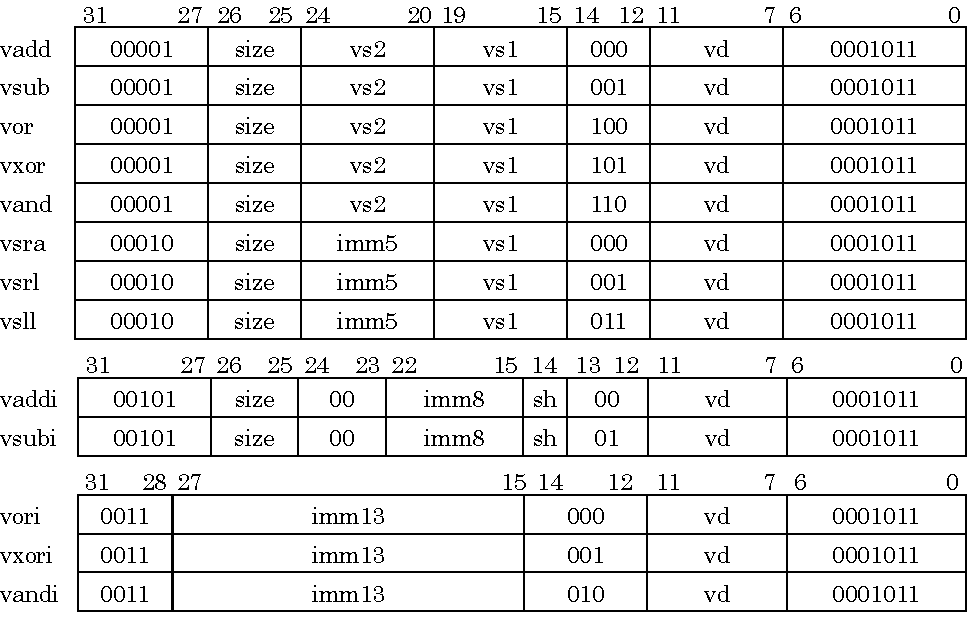
\includegraphics[scale=0.8]{image/jissou_inst_format.pdf}
    \caption{実装した命令}
    \label{fig:jissou_inst_format}
\end{figure}

図\ref{fig:jissou_inst_format}
vaddなどの命令フォーマットの26-25ビットにて指定されているsizeはベクトル要素のサイズを指定するためのフィールドであり,この値に応じたサフィックスが命令の末尾に追加されるものである.本研究では整数要素の処理の場合のみを想定し,このsizeの値は32ビットサイズを表すために'0b10'で固定している.また,即値を用いた算術演算命令であるvaddi,vsubiの命令フィールドのうち14ビットのshは24-20ビットで指定した即値を8ビットシフトするかを決定するためのフィールドである.このフィールドが0である場合はシフトを行わず,1であるときは8ビットのシフトを行う.このshの値はvaddi等の命令のオペランドにて指定を行うが,本研究ではシフトを行わない0で値を固定している.

実際に定義した命令フォーマットクラスの一覧を図\ref{fig:jissou_inst_format_class}
に示す.RVInstVVMIQSはvadd,vsub,vor,vxor,vandのための命令フォーマットで.RVInstIVIMIQSは5ビットの即値を用いるvsra,vsrl,vsll用の命令フォーマット,RVInstIVI8MIQSは8ビットの即値を用いるvaddi,vsubi用の命令フォーマット,RVInstIVI13MIQSは13ビットの即値を用いるvori,vxori,vandi用の命令フォーマットの定義である.

\begin{figure}[tb]
    \centering
    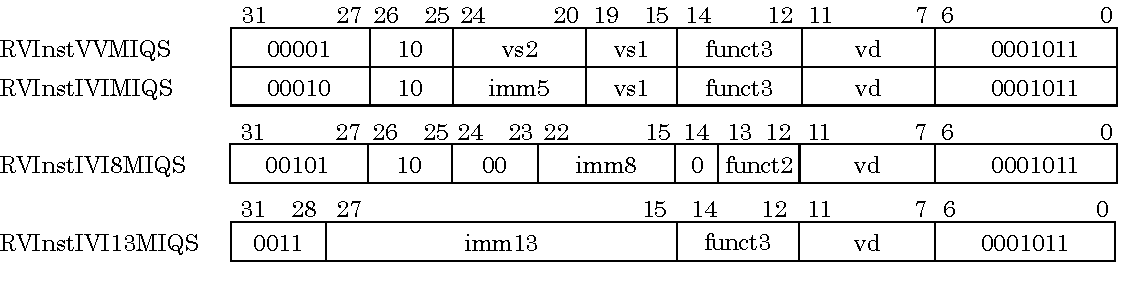
\includegraphics[scale=0.8]{image/jissou_inst_format_class.pdf}
    \caption{実装した命令フォーマットクラス}
    \label{fig:jissou_inst_format_class}
\end{figure}

また,実際のTableGenによる定義の例としてRVInstVVMIQSの定義を図\ref{fig:RVInstVVMIQS}
に示す.図\ref{fig:jissou_inst_format_class}
で示したフォーマットとなるように命令フィールドInstのどのフィールドにどの値が格納されるかを指定する.

\begin{figure}[tb]
    \centering
    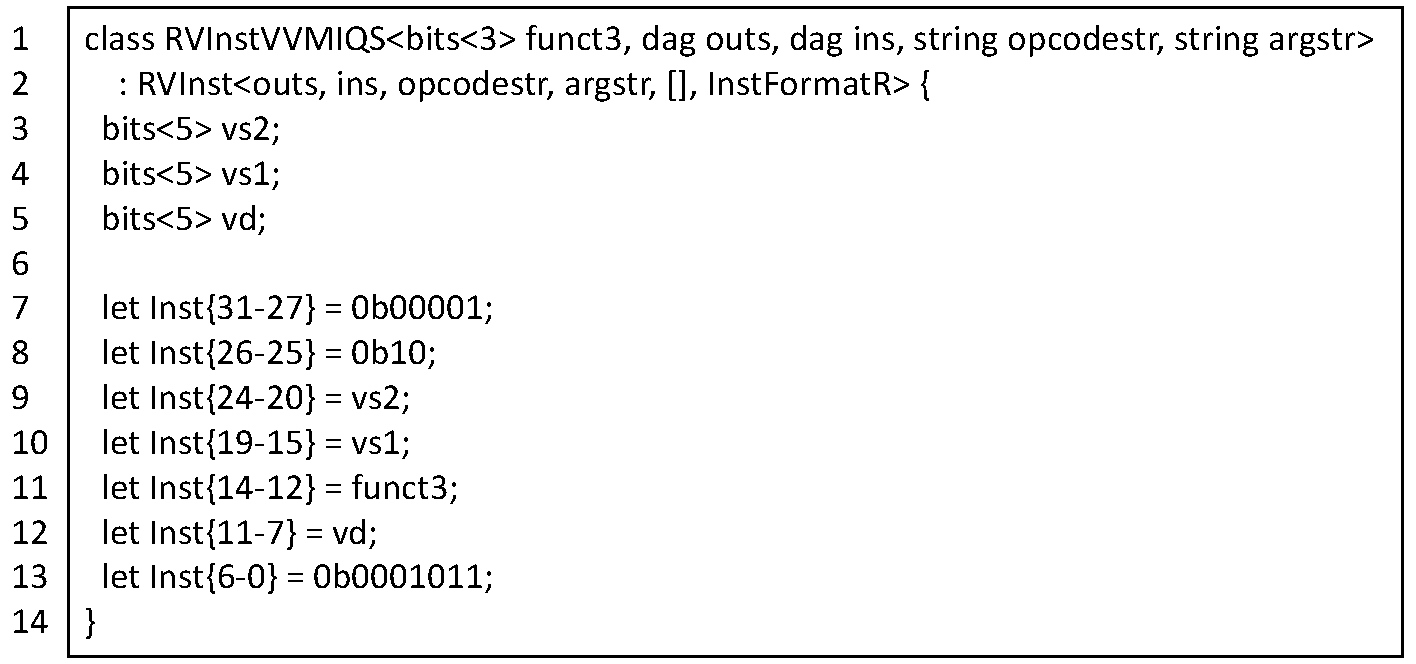
\includegraphics[scale=0.6]{image/RVInstVVMIQS_v2.pdf}
    \caption{TableGenによるRVInstVVMIQSの定義}
    \label{fig:RVInstVVMIQS}
\end{figure}

命令の定義を図\ref{fig:Inst_def}
に示す.
図\ref{fig:Inst_def}
のALUVVMIQSはベクトル同士の演算を行うための命令の定義用に定義の繰り返しを防ぐためのクラスである.ALUVVMIQSでは出力レジスタと入力レジスタの指定を行う.このクラスを定義することで例えば``vadd.w vd vs1 vs2''と``vsub.w vd vs1 vs2''のようにオペランドが同じ命令の定義を行う場合,ALUVVMIQSをインスタンス化する際に入出力レジスタの定義を繰り返しを防ぐことができる.

命令のインスタンス化も図\ref{fig:Inst_def}
で行っている.ベクトル算術・論理演算命令のインスタンス化を行っている.引数では命令の文字列と命令選択のための値を指定している.

\begin{figure}[tb]
    \centering
    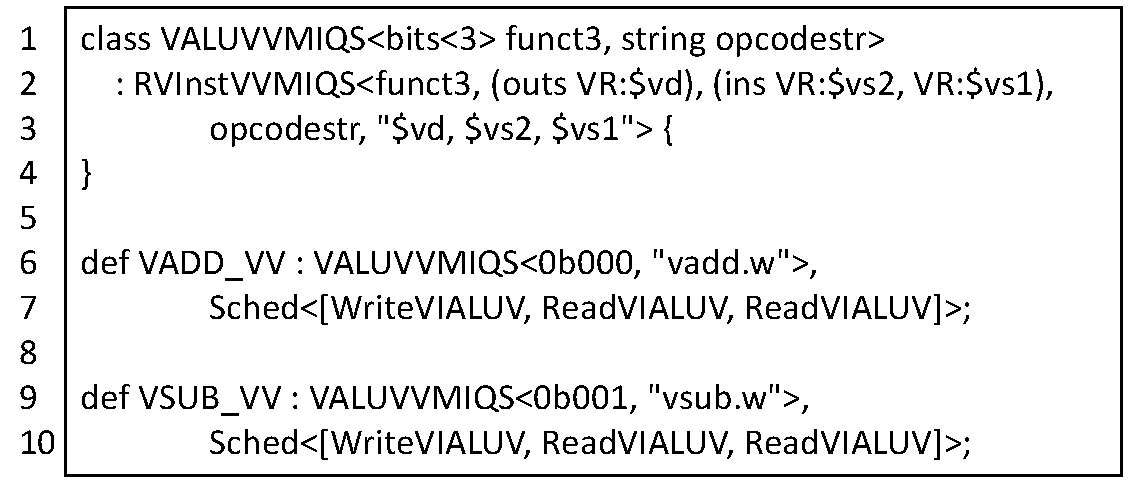
\includegraphics[scale=0.6]{image/Instruction_define.pdf}
    \caption{命令の定義}
    \label{fig:Inst_def}
\end{figure}

TableGenによる命令の定義は以上の様に行われ,残りの命令フォーマットや命令についても同様に定義を行った.

\newpage
\chapter{検証と課題}
\label{chp:5}
%5.tex
\ref{chp:5}章.終盤,もう少し.

\section{アセンブリコードの生成検証}
\label{chp:5_1}
%5_1.tex

実装した命令が正しく出力されるか,図%配列加算のCのソース
に示した配列加算のプログラムを入力としてアセンブリコードの出力を行った結果を図%Cのソースと一緒にする?別に?
に示す.


\section{課題}
\label{chp:5_2}
%5_2.tex

本研究ではベクトル拡張付きRISC-Vの命令の内,プレディケートなしのベクトル算術・論理演算命令,即値によるシフト命令を実装している.

図\ref{fig:add_array_c}
のアセンブリコードでもベクトルロード・ストア命令等の命令がRISC-VのV拡張の命令のままであり,ベクトル拡張付きRISC-V命令の内,ベクトルロード・ストア命令,プレディケート付きベクトル演算命令,ベクトル制御命令について未実装である.
これらの命令実装には本研究で行ったように命令の実装のみならず,新たなレジスタの定義に加えてLLVM IRへの変更が必要であると考えられる.

新たなレジスタの定義についてだが,これは未実装命令で用いられているプレディケートレジスタの定義が必要である.ベクトル拡張付きRISC-Vではプレディケートレジスタを用いたベクトル処理を行うことによってスケーラブルなベクトル拡張を実現している.そのためプレディケートレジスタが必須であるがRISC-Vはプレディケートレジスタを有していない.
そのため,新たにプレディケートレジスタを定義する必要がある.また,定義したプレディケートレジスタをそれを用いる命令のオペランドに割りあてられるようにするなど,命令とレジスタの定義のみでは実装が難しい.

また,LLVMによる自動ベクトル化が行われたLLVM IRではベクトル処理がベクトル演算の繰り返しと余りの要素の処理で行われているのに対して,我々のベクトル拡張付きRISC-Vではプレディケートレジスタを用いたベクトル処理を行っており,余りの要素の処理はプレディケートレジスタを用いた計算を行っている.
そのため,現在のLLVM IRから我々のベクトル拡張のプレディケートレジスタを用いる命令を効果的に生成することができないため,ベクトル化されたLLVM IRについて変更が必要である.

%\fi
\newpage
\chapter{おわりに}
\label{chp:outro}
%おわりに

本論文では,スケーラブルなベクトル処理を実現したベクトル拡張付きRISC-V向けのアセンブリコードを得るための手法について検討した.

まずベクトル拡張付きRISC-Vプロセッサ,ベクトル拡張付きRISC-Vの概要について確認し,コンパイラ基盤であるLLVMにおけるコード生成について確認した.

LLVMでは入力ソースコードをLLVM独自の中間表現であるLLVM IRに変換し,LLVM IRからSelectionDAG,MachineCode,MCLayerを経てアセンブリコードを生成する.LLVMは機能の再利用ができるため,実装済みのRISC-V向けのコンパイラ機能を再利用して我々のベクトル拡張付きRISC-Vのアセンブリコードの生成を目指した.

また,LLVMでは入力ソースコードにおける繰り返し処理をベクトル化されたLLVM IRに変換する自動ベクトル化機能を持っている.ベクトル化されたLLVM IRではベクトル演算の繰り返しと余剰要素の演算によるベクトル処理を行っている.

LLVMバックエンドではドメイン固有言語であるTableGenによって命令やレジスタの情報が定義され,その定義に従ってアセンブリコードなどの生成が行われるため,我々のベクトル拡張付きRISC-Vの命令をLLVMのRISC-V向けバックエンドに定義した.
ベクトル拡張付きRISC-Vの命令の内,プレディケートレジスタを用いないベクトル命令としてベクトル算術論理演算命令であるvadd,vsub,vand,vor,vxorと即値による演算命令であるvaddi,vsubi,vandi,vori,vxori,vsll,vsra,vsrlを実装した.


また,実装した命令のアセンブリコードが正しく生成されるかを実際に配列加算等の命令を入力として生成を検証した.

今後の課題としては,現時点では未実装である命令の実装を行い,動作可能なアセンブリコードを得ることを確認することが挙げられる.


\newpage
\acknowledgement
本研究の機会を与えていただき,
また,日頃から貴重な御意見,御指導いただいた,
大津 金光教授,横田 隆史教授,小島 駿助教授に深く感謝致します.
そして,本研究において多大な御力添えを頂いた,
木村 嘉毅氏をはじめとする
研究室の方々に感謝致します.


\endacknowledgement

\newpage
\thebibliography{99}
\bibitem{bib:fpga}
{\small 三好健文 : % 丁寧
%{\small 氏名ほか:             % スペースが足りない場合
\newblock ``FPGA 向けの高位合成言語と処理系の研究動向,''
\newblock コンピュータソフトウェア. 
\newblock Vol.30,
\newblock No.1,
\newblock pp.76-84,}
\newblock 2013.}

\bibitem{bib:2}
{\small Samuel Williams, et al.: % 丁寧
%{\small 氏名ほか:             % スペースが足りない場合
\newblock ``Roofline: an insightful visual performance model for multicore architectures,''
\newblock Communications of the ACM. 
\newblock Vol.52,
\newblock No.4,
\newblock pp.65-76,}
\newblock 2009.}

\bibitem{bib:ipa}
{\small 独立行政法人情報処理推進機構 社会基盤センター: % 丁寧
%{\small 氏名ほか:             % スペースが足りない場合
\newblock ``2020年度組込み/IoT産業の動向把握等に関する調査,''
\newblock 2021.}
\endthebibliography

\end{document}
